\documentclass{article}
\usepackage{tikz}
\usepackage{float}
\usepackage{amsmath}
\usepackage{lmodern}
\usepackage{amssymb}
\usetikzlibrary{calc}
\usetikzlibrary{hobby}
\usetikzlibrary{decorations.markings}
\usetikzlibrary{patterns, patterns.meta}
\usetikzlibrary{shapes}

\begin{document}

\centering

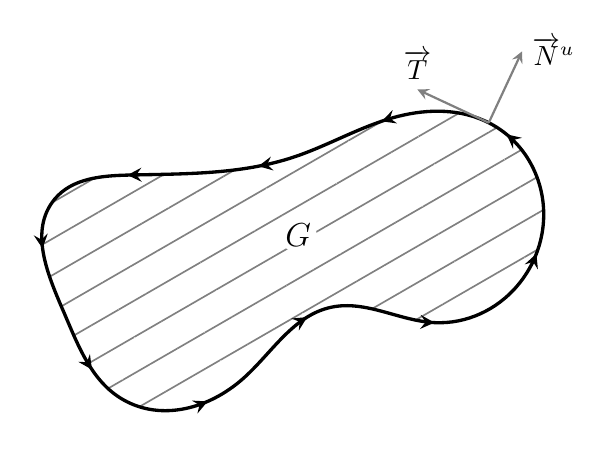
\begin{tikzpicture}
% define styles used in this picture
\tikzset{
BigTextFont/.style={font=\large},
every node/.style={font=\normalsize, text=black},
arrowstyle/.style={->, >=stealth}}

% waypoint coordinates (in degrees, as seen from origin)
\begin{scope}[scale=1.4, rotate=10]
       \coordinate (10degrees) at (1.2,0.3);     
       \coordinate (25degrees) at (2.0,0.5); 
       \coordinate (35degrees) at (2.3,1.6);
       \coordinate (50degrees) at (2.0,2.0);
       \coordinate (60degrees) at (1.2,2.2);
       \coordinate (85degrees) at (0.2,2.0);
       \coordinate (120degrees) at (-1.3,2.1);
       \coordinate (135degrees) at (-2.0,2.0);
       \coordinate (155degrees) at (-2.1,1.0);
       \coordinate (185degrees) at (-1.7,0.1);
       \coordinate (250degrees) at (-0.6,0.1);
       \coordinate (270degrees) at (0.3,0.6);
\end{scope}

% pattern on area
\fill[pattern={Lines[angle=30, distance=0.4cm, line width=0.6pt]}, pattern color=gray] (10degrees) to[closed, curve through =
{(25degrees) (35degrees) (50degrees) (60degrees) (85degrees) (120degrees) (135degrees) (155degrees) (185degrees) (250degrees)}] (270degrees);

% drawing area
\draw[postaction={decorate}, decoration={
       markings,
       mark = between positions 0.0 and 1 step 0.10 with {\arrow{stealth}},
       }]
[very thick] (10degrees) to[closed, curve through =
{(25degrees) (35degrees) (50degrees) (60degrees) (85degrees) (120degrees) (135degrees) (155degrees) (185degrees) (250degrees)}] (270degrees);

% G symbol
\node[draw=white, ellipse, inner sep=0, fill=white, BigTextFont, above] at (-0.15, 1.6) {$G$};

% CHECK
%plotting the waypoints
%\foreach \c in {(10degrees), (25degrees), (35degrees), (50degrees),
% (60degrees), (85degrees), (120degrees), (135degrees), (155degrees), (185degrees), (250degrees), (270degrees)} \fill[red] \c circle (1.0mm);

% Tangent and N^u
\pgfmathsetmacro{\TangentAngle}{155}             % Angle of the tangent
\pgfmathsetmacro{\NormalAngle}{\TangentAngle-90} % Angle of normal
\pgfmathsetmacro{\VectorSize}{1.0}               % Size of vector
\coordinate (Point) at (50degrees);              % Starting point
\coordinate (NormalEnd) at ($(Point)+(\NormalAngle:\VectorSize)$);
\coordinate (TangentEnd) at ($(Point)+(\TangentAngle:\VectorSize)$);
\draw[postaction={decorate}, decoration={
       markings,
       mark=at position 1.0 with {\node[right, black] {$\overrightarrow{N}^u$};}, 
       }]
[arrowstyle, gray, thick] (Point) -- (NormalEnd);
\draw[postaction={decorate}, decoration={
       markings,
       mark=at position 1.0 with {\node[above, black] {$\overrightarrow{T}$};}, 
       }]
[arrowstyle, gray, thick] (Point) -- (TangentEnd);

\end{tikzpicture}

\end{document}